\chapter{Introduzione}
\label{ChIntro}
%----------------------------------------------------------------------------------------

\section{High Performace Computing per Exascale}
%Exascale computing refers to computing systems capable of calculating at least 1018 floating point operations per second (1 exaFLOPS).
Nel contesto odierno di incredibile sviluppo tecnologico, alcuni calcolatori 
come il supercomputer Fugako giapponese \footnote{con 7,630,848 cores A64FX 48C da 2.2GHz},
hanno raggiunto performance di picco superiori a 1 Exaflops/s 
\footnote{in precisione singola o ulteriormente ridotta con il benchmark HPL-AI}
 ovvero $10^{18}$ operazioni floating point per secondo.\\
\voidLine
Risultati incredibili come questo sono legati alle enormi potenzialità offerte dal Hardware moderno,
che devono essere correttamente sfruttate dal Software eseguito, 
in particolar modo riguardo il livello di parallelismo offerto.\\

\subsection{Necessità di multi/many core nei calcolatori moderni}
%possibilità di creare core ancora più veloce
Il progresso tecnologico odierno nella integrazione dei componenti dei processori
ha raggiunto un livello tale da consentire, a livello teorico, la creazione di unità di calcolo 
ulteriormente più dense di transistor (e quindi inderettamente più veloci) di quelle attualmente in commercio,
ma non realizzabili a causa del surriscaldamento che verrebbe generato durante il loro utilizzo.\\
%intel slide compare power densisty
Per avere un'idea del problema del surriscaldamento nei processori,
è possibile analizzarne la densità di potenza $\left[\frac{W}{cm^2}\right]$
comparandola con le densità raggiunte da altre entità come in figura \ref{fig:powerDensityVSCriticalDim}.
\begin{figure}[H]
  \centering 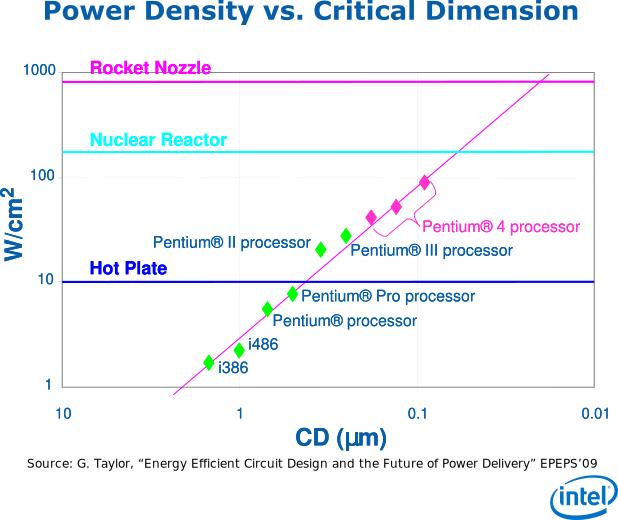
\includegraphics[width=.5\linewidth,keepaspectratio]{powerDensityVSCriticalDim.svg.png}
  \caption[densità di potenza CPU vs dimensione critica]{Comparazione tra la densistà di potenza di alcuni dispositivi tecnologici con dei processori intel rispetto alla loro dimensione critica,
			è possibile notare come la i valori raggiunti da alcuni modelli pentium si avvicinino a quelli di un reattore nucleare}
  \decoRule \label{fig:powerDensityVSCriticalDim}
\end{figure}
%%
\voidLine
%https://en.wikipedia.org/wiki/Processor_power_dissipation
Una buona approssimazione della potenza dissipata da un processore è data da:
$P_{cpu} =  P_{dyn} + P_{sc} + P_{leak}$ dove 
\begin{enumerate}
	\item $P_{dyn}\quad$ modella la dissipazione di energia dovuta all'attività interna dei gate logici della CPU,
	approssimabile con $P_{dyn} = CV^2 f$
	\item $P_{sc}\quad$	 modella la dissipazione di energia 
	dovuta ad un collegamento diretto che si può creare tra la sorgente di energia e il ground durante
	un cambiamento di stato di un gate CMOS
	\item $P_{leak}\quad$ modella le perdite di energia intrinseche dei singoli transistors.
\end{enumerate}
Dato che la frequenza di lavoro dell'unità di calcolo è proporzionale ai punti 1 e 2,
è necessario limitarla, purtroppo, per evitare un surriscaldamento critico dei componenti elettronici.\\
Indirettamente, questo comporta la necessità di limitare anche le potenzialità offerte da 
una singola unità di calcolo.
\voidLine
La soluzione per far fronte a questa limitazione fisica/tecnologica per poter
costruire processori più performanti è quella di realizzare CPU con diverse unità di calcolo separate o core.\\
%SW parallelo che sfrutti i diversi core
In questo contesto si inserisce il calcolo parallelo, ovvero delle tecniche per realizzare software che 
sfrutti la disponibilità dei vari core del calcolatore mediante un partizionamento del lavoro in parti
assegnabili alle singole unità di calcolo.\\
%TODO HPC in generale... ===> targets, ... TODO ?
%\subsection{High Performance Computing}
L'High Performance Computing si riferisce a tecnologie hardware e software 
usate per realizzare sistemi di elaborazione ad alte prestazioni 
per applicazioni che richiedono computazioni molto onerose, non risolvibili con sistemi informatici tradizionali.\\

\section{Uso di Metodi basati su Algebraic Multi Grid nel calcolo scientifico} \label{chIntro:PDE_intro}
Applicazioni HPC tipiche sono provenienti dal mondo ingegneristico e dal calcolo scientifico,
come ad esempio la risoluzione di equazioni differenziali alle derivate parziali (\emph{PDE}) su dominii 2D o 3D.\\
Le PDE sono usate per descrivere moltissimi fenomeni fisici relativi alla
dinamica dei fluidi, alla meccanica quantistica e chimica computazionale % e molti altri derivanti da applicazioni ingegneristiche, %TODO MORE
così come vari problemi nell'area dell'ingegneria, biologia e economia.\\
Dato che molto spesso non esistono soluzioni esplicite in forma chiusa a queste equazioni,
vengono calcolate soluzioni approssimante ottenute da tecniche numeriche.\
Molte tecniche numeriche per risolvere delle PDE trasformano le equazioni differenziali
in equazioni algebrice, mediante un processo di discretizzazione delle equazioni nel dominio del problema da risolvere.\\
Conseguentemente un problema ricorrente in varie applicazioni algebriche e nel calcolo scientifico in generale, 
%come gia menzianto %in \ref{chIntro:},
è risolvere sistemi sparsi di dimensioni grandi derivanti da metodi di risoluzione numerici di PDE.\\
\voidLine
Il sistema lineare sparso di riferimento che verrà usato nel seguito è 
\begin{equation} \label{eq:1}
Ax=b
\end{equation}
dove $A$ è una matrice sparsa di grandi dimensioni,
simmetrica e definita positiva \emph{s.p.d.}\\
\subsection{Importanza della sparsità delle matrici}
%sparsity defs
La proprietà di sparsità della matrice $A$  nel sistema \ref{eq:1}, ovvero la proprietà di avere per la maggioranza degli elementi il valore zero,
%Since differential surface properties are defined locally, the discretization of PDEs typically leads to sparse linear systems, in which the ith row contains non- zeros only in those entries corresponding to the geodesic or topological neighbor- hood of vertex xi . We are therefore interested in solvers that exploit this sparsity in order to minimize both memory consumption and computation times. 
deriva dalla discretizzazione delle PDE nel problema originario in una mesh di punti \cite{sparseLinearSolverTR}.
Una caratteristica comune nei metodi di discretizzazione utilizzabili come differenze finite, elementi finiti e volumi finiti 
è che il numero di elementi in ogni equazione discretizzata dipende da proprietà topologiche locali alla discretizzazione
e non dalla dimensione globale del dominio del problema da risolvere \cite{spMVfanf,pdeSparsfd1,pdeSparsfd2,pdeSparsfd3}.
Conseguentemente la matrice generata da questi metodi è comunemente sparsa.\voidLine
La proprietà di sparsità di $A$ consente l'utilizzo di rappresentazioni idonee in memoria durante il calcolo, 
dove vengono salvati solamente gli elementi non zero.\\
Formati tipici di memorizzazione per matrici sparse sono: \emph{CompressedSparseColumn, CompressedSparseRow, Ellpack, DIA}.%\\DD
\voidLine	%sparsity advantage
Sfruttare la sparsità delle matrici nella risoluzione di un problema come \ref{eq:1}, consente di ottenere svariati vantaggi
rispetto ad usare le tecniche convenzionali dell'algebra lineare densa, come un utilizzo molto più efficiente della memoria.\\
Spingendo al limite le potenzialità dei super calcolatori attuali e cercando soluzioni sempre più accurate ai problemi moderni di calcolo scientifico,
si rende indispensabile sfruttare questa proprietà quando presente,
dato che tecniche classiche per matrici dense necessiterebbero di una quantità di memoria 
quadratica nella dimensione della matrice, contro una quantità lineare nel numero dei non zeri con tecniche di algebra sparsa.
\voidLine	%prefer of iterative solver to keep sparsity
\subsection{Tecniche risolutive efficienti di sistemi sparsi} \label{directVsIndirectSpLinSysSolvers}
Solutori di sistemi come \ref{eq:1}, possono essere di tipo diretto o iterativo.\\
I solutori di tipo diretto tipicamente impiegano una fattorizzazione della matrice $A$ 
in matrici di struttura semplice (triangolare, diagonale, ortogonale),
per poi applicare operazioni che portano alla soluzione del sistema $x^{\ast}$.\\
I solutori di tipo indiretto generano una sequenza di soluzioni intermedie,
(ipoteticamente) %TODO
convergenti alla soluzione del sistema $x^{\ast}$.\\
Una differenza significativa tra le due classi di soluzioni 
è che i solutori diretti non sfruttano la sparsità della matrice in input
nei passaggi intermedi.
Infatti, in misura differente in base al metodo di risoluzione diretto utilizzato,
la fattorizzazione della matrice può portarne alla perdita della proprietà di sparsità %e divenire densa
come mostrato dalla figura \ref{fig:Efficient_Linear_System_Solvers_for_Mesh_Processing_densificationByDirectSolver}.\\
\begin{figure}[H]
  \centering 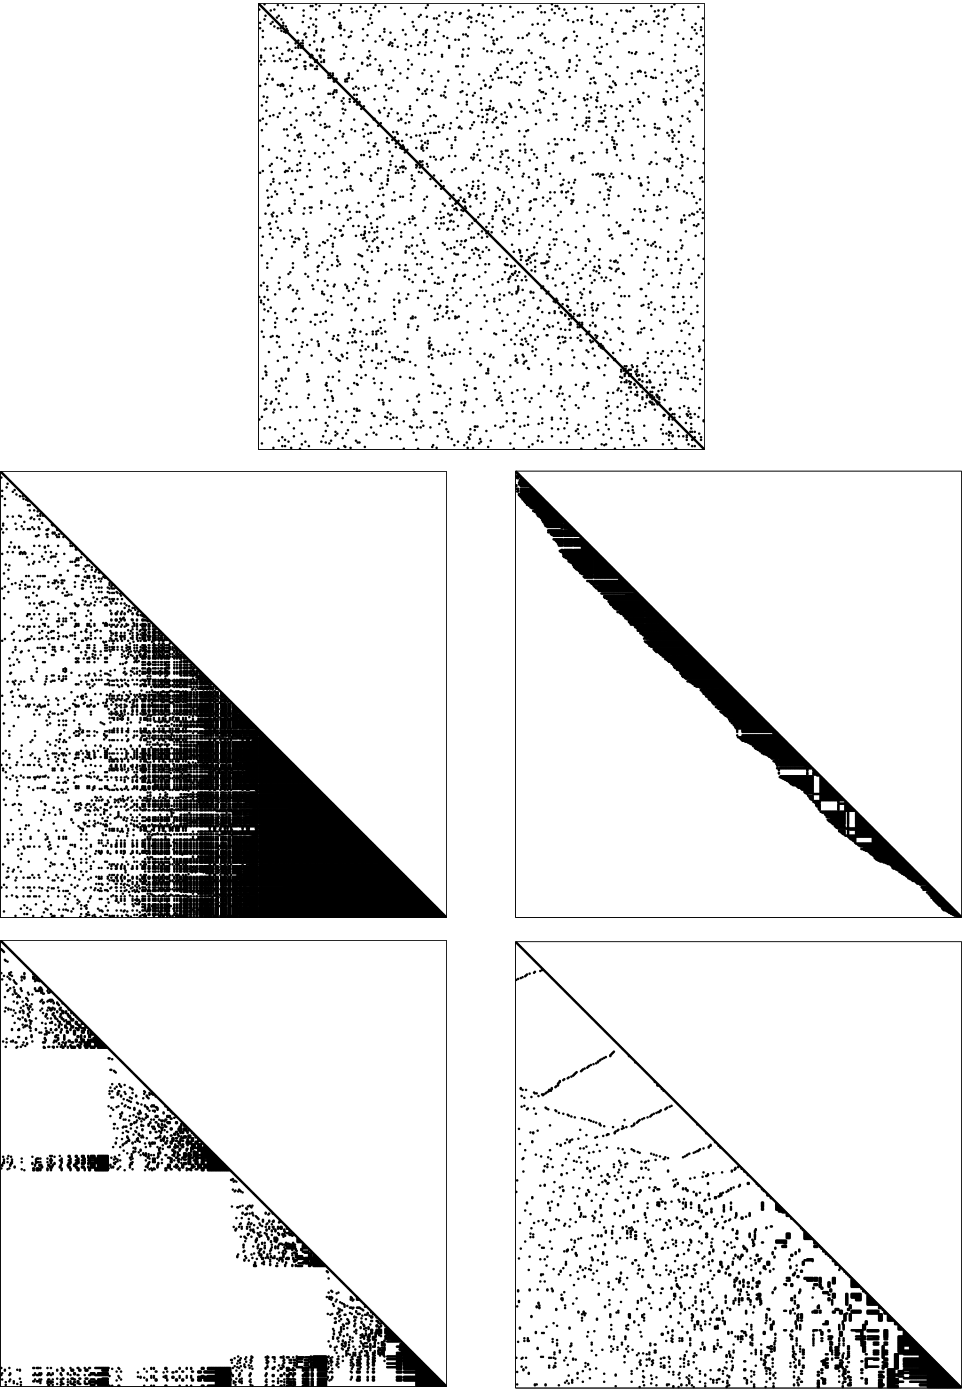
\includegraphics[height=.77\linewidth,keepaspectratio]{Efficient_Linear_System_Solvers_for_Mesh_Processing_densificationByDirectSolverSimplied.svg.png}
  \captionsetup{singlelinecheck=off}
  \caption[perdità di sparsità nelle matrici fattorizzate da solutori diretti]
	{Varie fattorizzazioni di una matrice altamente sparsa A 500x500 con soli 3502 elementi \nnz (in alto)
				in  matrici con un numero di \nnz incrementato a vari livelli  \cite{sparseLinearSolverTR}:
				\begin{itemize}
					\item	36000 \nnz con il metodo di \emph{Cholesky} 				in alto a sinistra 
					\item	14000 \nnz con il metodo di \emph{Cuthill-McKee}			in alto a destra
					\item	 6203 \nnz con il metodo \emph{minimum degree ordering}		in basso a destra
					\item	 7142 \nnz con il metodo \emph{nested dissection method}	in basso a sinistra
				\end{itemize}
  }
  \decoRule \label{fig:Efficient_Linear_System_Solvers_for_Mesh_Processing_densificationByDirectSolver}
\end{figure}
%Fig. 2. The top row shows the non-zero pattern of a typical 500 × 500 matrix A and its Cholesky factor L, corresponding to a Laplacian system on a triangle mesh. Although A is highly sparse (3502 non-zeros), the factor L is dense (36k non-zeros). The reverse Cuthill-McKee algorithm minimizes the envelope of the matrix, resulting in 14k non-zeros of L (2nd row ). The minimum degree ordering avoids fill-in during the factorization, which decreases the number of non-zeros to 6203 (3rd row ). The last row shows the result of a nested dissection method (7142 non-zeros), that allows for parallelization due to its block structure. 
Di contro a questa penalità dei solutori diretti, c'è il vantaggio che la fattorizzazione della matrice $A$, 
può essere riutilizzata per sistemi in cui viene cambiato il lato destro di \ref{eq:1},
%o anche in caso in cui la matrice $A$ cambia i valori \nnz ma non il loro pattern di sparsità... 50% del tempo
come analizzato in \cite{sparseLinearSolverTR}.\\
\voidLine
\subsection{Solutori MultiGrid} \label{multiGrid}
Tra i solutori iterativi più efficienti ci sono quelli basati su metodi \emph{MultiGrid}, 
che godono di ottime caratteristiche di scalabilità come avere un numero di iterazioni e 
un costo per iterazione approssimatamente costante all'incrementare della dimensione del problema \cite{AMGgeneralANY,Sp3MM4AMG}.\\
%MultiGrid in generale-wikipedia
L'idea principale dei metodi MultiGrid è quella di 
risolvere il sistema \ref{eq:1} iterativamente, applicando una serie di correzioni 
alle soluzioni approssimate ottenute con un metodo iterativo basico.\\
Le correzioni sono applicate ai residui associati agli errori delle soluzioni intermedie approssimate,
risolvendo un sotto problema dell'originale contente un sottoinsieme delle incognite.\\ %, a grana meno fine
Il sotto problema può essere risolto a sua volta applicando ricorsivamente delle correzioni
a dei sotto problemi ulteriori, sempre più piccoli e facili da risolvere,
fino a quando la risoluzione dell'ultimo sotto problema è di una difficoltà trascurabile 
rispetto a generarne un altro.\\
\voidLine
%tipi di shape per iterazioni
Le iterazioni di questi metodi possono essere strutturati con cicli di varia natura.
Tra le metodologie principalmente utilizzati ci sono cicli a forma V, F e W.\\
%In figura \ref{fig:Multigrid_Visualization_wikipedia} è disponibile una rappresentazione schemativa di un algoritmo MultiGrid iterativo con un ciclo-V.
\begin{figure}[H]
  \centering \includegraphics[width=.84\linewidth,keepaspectratio]{Multigrid_Visualization_wikipedia.png}
  \caption[ciclo V di un Multigrid] {Rappresentazione grafica di un ciclo V di un solutore MultiGrid}
  \decoRule \label{fig:Multigrid_Visualization_wikipedia}
\end{figure}

%\par\null\par	%GMG vs AMG
Tra i principali tipi di metodi MultiGrid disponibili ci sono quelli di tipo Geometrico (\emph{GMG}) e quelli di tipo Algebrico (\emph{AMG}).
La differenza sostanziale è il modo di determinazione dei sotto problemi intermedi da risolvere ad ogni iterazione.\\
Nei metodi Geometrici, si usa una gerarchia di griglie iterativamente più sparse, %TODO derivate da quella di discretizzazione originale,
derivate da informazioni sulla struttura della griglia di discretizzazione originaria.\\
%One main component of this type of multilevel algorithm is a hierarchy of geomet- ric grids, typically a sequence of nested grids obtained by successive refinement. The resulting algorithms are known as geometric multigrid (GMG) methods. 
%AMG finally!
I metodi Algebrici riescono ad utilizzare unicamente informazioni derivanti dalla matrice associata al sistema da risolvere \ref{eq:1},
pur mantenendo la stessa complessità asintotica dei \emph{GMG}.\\
%Qualunque problema discretizzato con delle griglie non strutturate, p.es. agli elementi finiti
Questa proprietà degl'\emph{AMG}, rende possibile applicarli 
alla risoluzione di problemi discretizzati con griglie non strutturate,
ad esempio mediante il metodo degli elementi finiti.\\
\cite{AMGgeneralANY}.\\
\par\null\par	%GMG vs AMG
La gerarchia di sotto-problemi intermedi da risolvere ad ogni iterazione con i metodi AMG è derivata dal triplo prodotto di Galerkin:\\
\begin{equation} \label{eq:galerkin}
A_{l+i} = (P_l)^T \cdot A_l \cdot P_l~l=0,\dots,nl-1
\end{equation}
dove $A_0 = A$ \cite{AMG4PSBLAS} e $P_l$ è una sequenza di matrici di prolungamento $n_l \times n_{l+1}$ con $n_0=n$ e $n_{l+1}<n_l$.\\
%TODO more?
\par\null\par
%actual time costs :((( , previous prof notes 
%%Non esattamente: di quale algoritmo iterativo stiamo parlando? 
%% Il triplo prodotto viene eseguito durante la costruzione della gerarchia, non durante la applicazione della gerarchia stessa all'interno dell'algoritmo iterativo di soluzione del sistema lineare.
%%E tuttavia, il triplo prodotto è importante perchè il tempo di costruzione del precondizionatore ne dipende. 
%%In generale, il tempo complessivo per un sistema lineare vale 
%%T_{tot} = T_{setup} + T_{it}\times N_{it} 
%%ed il triplo prodotto entra nel tempo di setup. 
%%Se un sistema  con la stessa matrice viene risolto più volte, il precondizionatore si riutilizza, e quindi il tempo di setup viene ammortizzato su più esecuzioni, il che vuol dire che ci si può permettere un setup più complesso.
In generale il tempo complessivo di risoluzione del sistema lineare con dei metodi AMG è  $T_{tot} = T_{setup} + T_{it}\cdot N_{it}$,
dove $T_{it}\cdot N_{it}$ è associato al costo delle iterazioni del metodo, 
mentre $T_{setup}$ comprende il calcolo di tutto il necessario all'esecuzioni delle iterazioni,
tra cui la costruzione della gerarchia di sotto problemi mediante il triplo prodotto.\\ %TODO setup of preconditioner https://en.wikipedia.org/wiki/Preconditioner#Description ?? 
\par\null\par
Realizzare il triplo prodotto tra matrici sparse, denominato \\{\bf{Sp}}arse{\bf{3}}{\bf{M}}atrixMatrix{\bf{M}}ultiplication (\emph{Sp3MM})
in parallelo è l'obbiettivo di questa tesi, al fine di potenziare progetti come \cite{AMG4PSBLAS} che sfruttano solutori basati su AMG.\\
%organizzazione seguito
%Il seguito della tesi è strutturato come segue
\section{Algebraic MultiGrid for Parallel Sparse BLAS} \label{amg4psblas}
PSBLAS è una libreria software che punta a consentire la realizzazione di varie applicazioni di calcolo scientifico computazionalmnte intense,
mediante implementazioni di risolutori iterativi per sistemi lineari sparsi 
usando il padarigma di programmazione per sistemi a memoria distribuita.\\
L'ambito di questa libreria è relativo alle PDE discretizzate mediante differenze finite o elementi finiti,
ma anche a problemi di ottimizzazione non lineare come problemi di controllo ottimo \cite{PSBLAS3man}.\\
AMG4PSBLAS \cite{AMG4PSBLASman} fornisce i metodi MultiGrid di tipo algebrico precedentemente descritti,
utilizzando come layer sottostante PSBLAS.\\
Il progetto Software è scritto in Fortran 2003, sfruttandone le possibilità di 
usare un design object-oriented degli algoritmi, mediante varie funzionalità disponibili nello standard del linguaggio,
consentendo un'ottima gestione delle varie implementazioni offerte. 
